% Block diagram for the README. Build with `make diagram`.
\documentclass[tikz, border=0pt]{standalone}
\usepackage[T1]{fontenc}
\usepackage{newtxtext,newtxmath}
\usetikzlibrary{calc, backgrounds}

\begin{document}
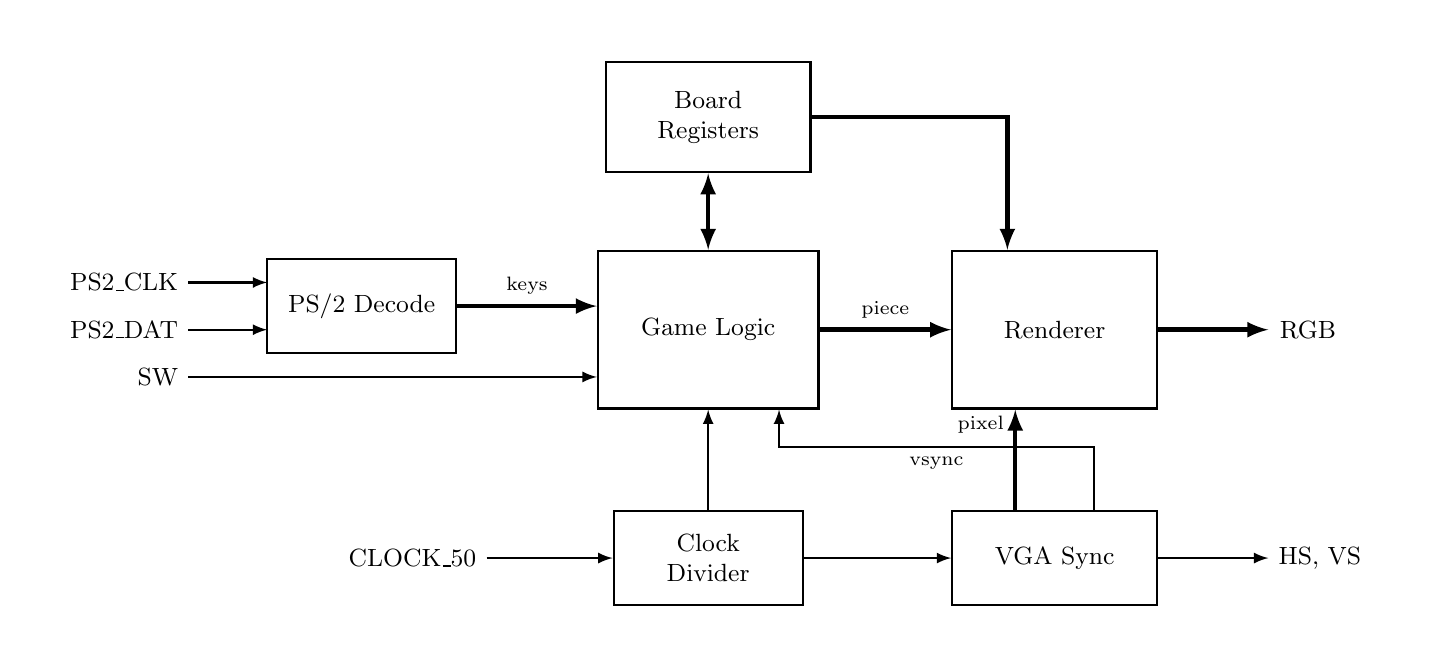
\begin{tikzpicture}[
    show background rectangle,
    background rectangle/.style={fill=white},
    inner frame sep=12pt,
    font=\small,
    blk/.style={draw, thick, align=center, minimum height=1.2cm},
    sig/.style={-latex, thick},
    bus/.style={-latex, line width=1.6pt},
    lab/.style={font=\scriptsize},
  ]
  \node[blk, minimum width=2.4cm] (ps2)  at (0,0.3)  {PS/2 Decode};
  \node[blk, minimum width=2.8cm, minimum height=2.0cm] (game) at (4.4,0) {Game Logic};
  \node[blk, minimum width=2.6cm, minimum height=1.4cm] (brd)  at (4.4,2.7) {Board\\Registers};
  \node[blk, minimum width=2.6cm, minimum height=2.0cm] (rend) at (8.8,0) {Renderer};
  \node[blk, minimum width=2.6cm] (vga)  at (8.8,-2.9) {VGA Sync};
  \node[blk, minimum width=2.4cm] (div)  at (4.4,-2.9) {Clock\\Divider};

  \draw[sig] (-2.2,0.6) node[left] {PS2\_CLK} -- (-1.2,0.6);
  \draw[sig] (-2.2,0.0) node[left] {PS2\_DAT} -- (-1.2,0.0);
  \draw[sig] (-2.2,-0.6) node[left] {SW} -- (game.west |- 0,-0.6);
  \draw[sig] (div.west) ++(-1.6,0) node[left] {CLOCK\_50} -- (div.west);

  \draw[bus] (ps2.east) -- node[above, lab] {keys} (game.west |- ps2.east);
  \draw[bus, latex-latex] (game) -- (brd);
  \draw[bus] (brd.east) -| ([xshift=-0.6cm]rend.north);
  \draw[bus] (game) -- node[above, lab] {piece} (rend);
  \draw[sig] (div) -- (vga);
  \draw[sig] (div) -- (game);
  \draw[bus] ([xshift=-0.5cm]vga.north) -- node[left, lab, pos=0.85] {pixel} ([xshift=-0.5cm]rend.south);
  \draw[sig] ([xshift=0.5cm]vga.north) -- ++(0,0.8) -| ([xshift=0.9cm]game.south)
    node[pos=0.25, below, lab] {vsync};

  \draw[bus] (rend.east) -- ++(1.4,0) node[right] {RGB};
  \draw[sig] (vga.east) -- ++(1.4,0) node[right] {HS, VS};
\end{tikzpicture}
\end{document}
